\newpage
\criteria{Facilities and Infrastructure}

\subcriteria{The physical resources to deliver the curriculum, including equipment, material, and information technology, are shown to be sufficient.}

หลักสูตรวิทยาศาสตรบัณฑิต สาขาวิชาคณิตศาสตร์ประยุกต์  ใช้ทรัพยากรกายภาพและสิ่งสนับสนุนการเรียนรู้ของคณะและมหาวิทยาลัยในการจัดการเรียนการสอน โดยมีรายละเอียดดังนี้
\begin{enumerate}
\item {\bf ห้องเรียนสำหรับการเรียนการสอน:}\\ มหาวิทยาลัยและคณะมีการจัดเตรียมห้องเรียนเพื่อรองรับการจัดการเรียนการสอนทั้งในรูปแบบ Onsite และ Online ที่พร้อมวัสดุอุปกรณ์เทคโนโลยีและอินเทอร์เน็ต ซึ่งในห้องเรียนแต่ละห้องจะประกอบไปด้วยอุปกรณ์ในการเรียนการสอน คอมพิวเตอร์ เครื่องฉายและจอโปรเจคเตอร์ ไมโครโฟน ลำโพง ที่พร้อมใช้งาน ในกรณีจัดการเรียนการสอนในรูปแบบ Online อาจารย์ผู้สอนสามารถใช้โปรแกรม Microsoft Teams เป็นโปรแกรมหลักในการจัดการเรียนการสอน Online นอกจากนี้ในส่วนของสาขาวิชาได้จัดหาโปรแกรม Zoom ลิขสิทธิ์ ไว้บริการให้กับอาจารย์ในสาขาวิชา  นอกจากนั้นระบบอินเทอร์เน็ตสามารถเชื่อมต่อได้ทุกห้องเรียนทั้งระบบ LAN และสัญญาณอินเทอร์เน็ตไร้สาย (Wi Fi) ทั้งนี้ในกรณีอุปกรณ์ต่างๆ ในห้องเรียนมีปัญหา อาจารย์สามารถติดต่อฝ่ายอาคารสถานที่ของคณะที่ดูแลรับผิดชอบ ผ่านทางโทรศัพท์ซึ่งมีการแจ้งหมายเลขติดต่อไว้ในทุกห้องเรียน เพื่อมาช่วยแก้ไขปัญหาให้แก่อาจารย์ได้ สำหรับห้องเรียนและห้องปฏิบัติการในความรับผิดชอบของหลักสูตรที่ใช้ในการจัดการการเรียนการสอนในรายวิชาชีพและรายวิชาศึกษาทั่วไป (บางกลุ่ม) เป็นห้องเรียนจำนวน 3 ห้องและห้องปฏิบัติการจำนวน 3 ห้อง รายละเอียดดังตาราง \\
{\tiny
\begin{center}
	\begin{tabular}{|c|l|cc|c|}
	%	\caption{ห้องเรียนห้องปฏิบัติการของสาขาวิชาคณิตศาสตร์}
	%	\label{Table:7.1-1}\\
		\hline
		\multirow{2}{*}{\textbf{ชื่ออาคาร}}                                                                      & \multicolumn{1}{c|}{\multirow{2}{*}{\textbf{ชื่อห้องเรียน/ห้องปฏิบัติการ}}} & \multicolumn{2}{c|}{\textbf{ประเภทห้อง}}                          & \textbf{ขนาดความจุ} \\ \cline{3-4} 
		& \multicolumn{1}{c|}{}                                                       & \multicolumn{1}{c|}{\textbf{ห้องเรียน}} & \textbf{ห้องปฏิบัติการ} &  \textbf{(คน)}               \\ \hline
		\begin{tabular}[c]{@{}c@{}}อาคารเฉลิมพระเกียรติ ๖ \\ รอบพระชนมพรรษา ชั้น 3\end{tabular}                  & ห้องบรรยายรวม ST-1 301     &  \multicolumn{1}{c|}{\checkmark}                   &                         & 80                  \\ \hline
		\multirow{5}{*}{\begin{tabular}[c]{@{}c@{}}อาคารเฉลิมพระเกียรติ ๖ \\ รอบพระชนมพรรษา ชั้น 9\end{tabular}} & \multicolumn{1}{c|}{ห้อง Research and Discussion ST-1 908}                  & \multicolumn{1}{c|}{}                   &     \checkmark                    & 20                  \\ \cline{2-5} 
		& ห้องปฏิบัติการคอมพิวเตอร์ ST-1 905                                          & \multicolumn{1}{c|}{}                   &\checkmark                         & 30                  \\ \cline{2-5} 
		& ห้อง Smart Class Room ST-1 906                                              & \multicolumn{1}{c|}{}                   &  \checkmark                       & 40                  \\ \cline{2-5} 
		& ห้องบรรยายรวม ST-1 910                                                      & \multicolumn{1}{c|}{\checkmark}                   &                         & 40                  \\ \cline{2-5} 
		& ห้องบรรยายรวม ST-1 911                                                      & \multicolumn{1}{c|}{\checkmark}                   &                         & 40                  \\ \hline
	\end{tabular}
\end{center}
}

%\end{table} 

%\includegraphics[width=0.9\textwidth]{Table 7.1-1.jpg}\\
\noindent
{\bf หมายเหตุ}	สำหรับรายวิชาศึกษาทั่วไป หลักสูตร ฯ ใช้ห้องเรียนที่อาคารปฏิบัติการเรียนรวม (รป.)
%\begin{figure}[h!]
\begin{center}
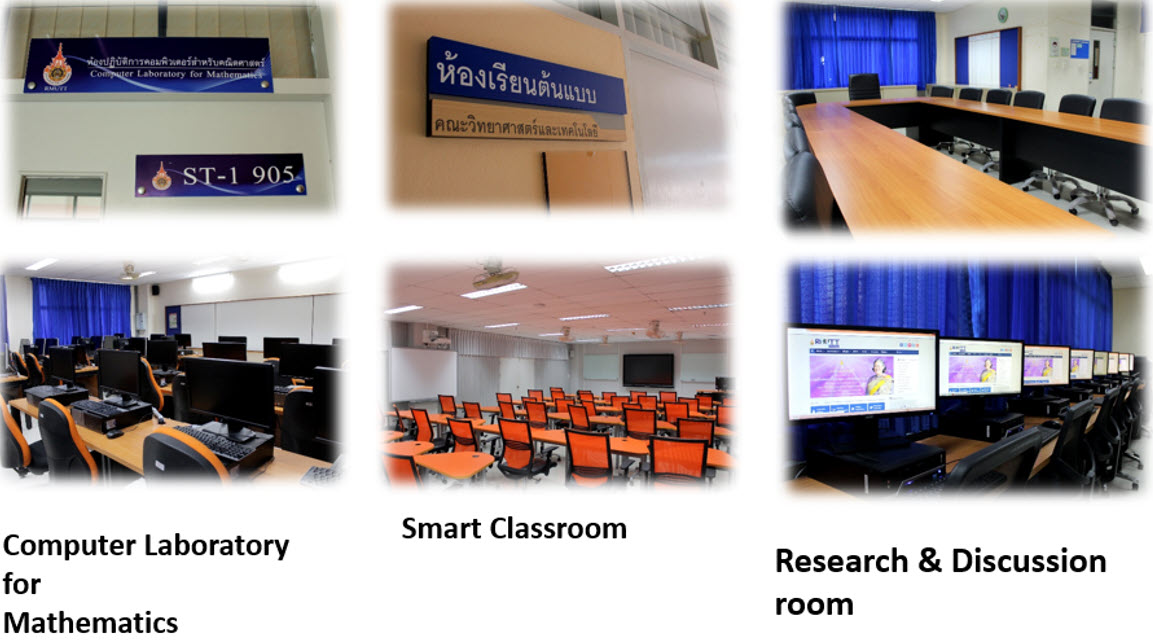
\includegraphics[width=0.8\textwidth]{Pic7.1-1.jpg}
\end{center}
%\caption{ห้องปฏิบัติการ ST-1 905, ST-1 906, ST-1 908  }
%\end{figure}
\item {\bf ห้องสมุด:}\\ {\bf ห้องสมุดของมหาวิทยาลัย} มีให้บริการหนังสือ วารสาร สื่อวิดีทัศน์ และอื่นๆ วารสารเฉพาะสำหรับหลักสูตร e-Databases e-Theses e-Newpapers ระบบสืบค้นข้อมูลทรัพยากรห้องสมุดผ่านระบบห้องสมุดอัตโนมัติ (Web OPAC) IT-Zone บริการสื่ออิเล็กทรอนิกส์ Edutainment ZONE บริการจองห้องออนไลน์ บริการวารสาร นิตยสาร หนังสือพิมพ์ บริการด้านภาษา/โปรแกรมการฝึกปฏิบัติ/ทดสอบทางภาษา (SPEEXX (CLT, Chiness Mandarin, Sanako, Euro Talk) เป็นต้น โดยห้องสมุดมหาวิทยาลัยมีพื้นที่ใช้สอย 20,000 ตารางเมตร มีหนังสือทั่วไปภาษาไทย 126,209 เล่ม หนังสือภาษาอังกฤษ 21,957 เล่ม วิทยานิพนธ์จำนวน 4,442 เล่ม งานวิจัย 4,892 เล่ม สื่ออิเล็กทรอนิกส์ 7,659 เล่ม  ฐานข้อมูล 19 ฐาน e-Book 5 ฐานข้อมูล โซนให้บริการชั้น 1 มีเครื่องคอมพิวเตอร์ให้บริการ 90 เครื่อง โซนอบรม e-library มีเครื่องคอมพิวเตอร์ให้บริการ 30 เครื่อง 
\begin{center}
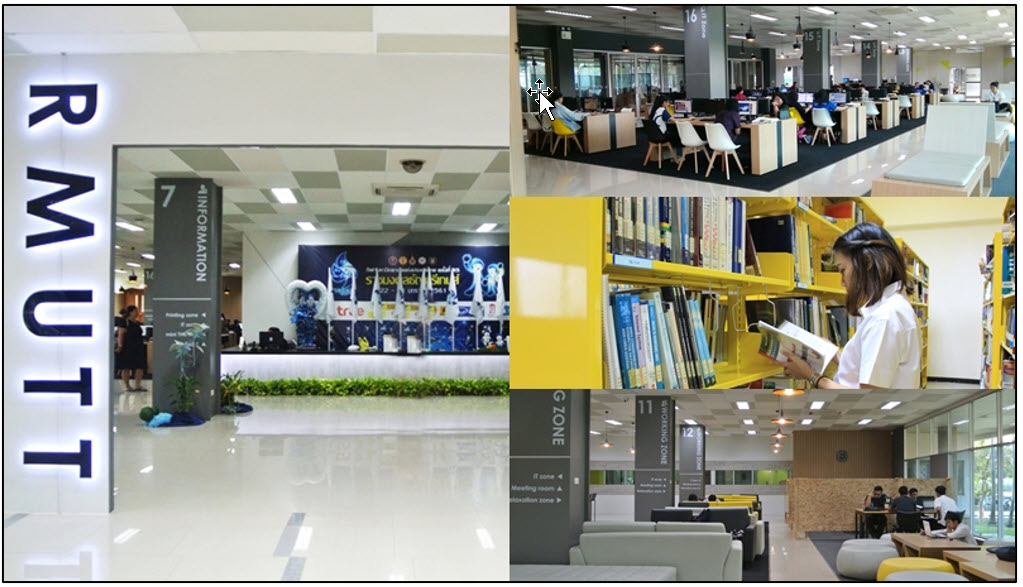
\includegraphics[width=0.8\textwidth]{Pic7.1-2.jpg}\\
\end{center}
{\bf ห้องสมุดคณะวิทยาศาสตร์และเทคโนโลยี มทร.ธัญบุรี} มีบริการยืมคืนหนังสือเฉพาะทางด้านวิทยาศาสตร์และเทคโนโลยีสำหรับนักศึกษาในสาขาวิชาต่าง ๆ (เป็นหนังสือภาษาไทย จำนวน 7,294 เล่ม หนังสือภาษาอังกฤษ จำนวน 1,184 เล่ม หนังสืออ้างอิงภาษาไทย จำนวน 11 เล่ม หนังสืออ้างอิงภาษาอังกฤษจำนวน 10 เล่ม หนังสือนวนิยาย จำนวน 39 เล่ม เรื่องสั้น จำนวน 15 เล่ม) บริการห้อง Discussion Room จำนวน 10 ที่นั่ง ณ ชั้น 4 ห้องสมุด คณะวิทยาศาสตร์และเทคโนโลยี มทร.ธัญบุรี บริการตอบคำถามและช่วยค้นคว้า
\begin{center}
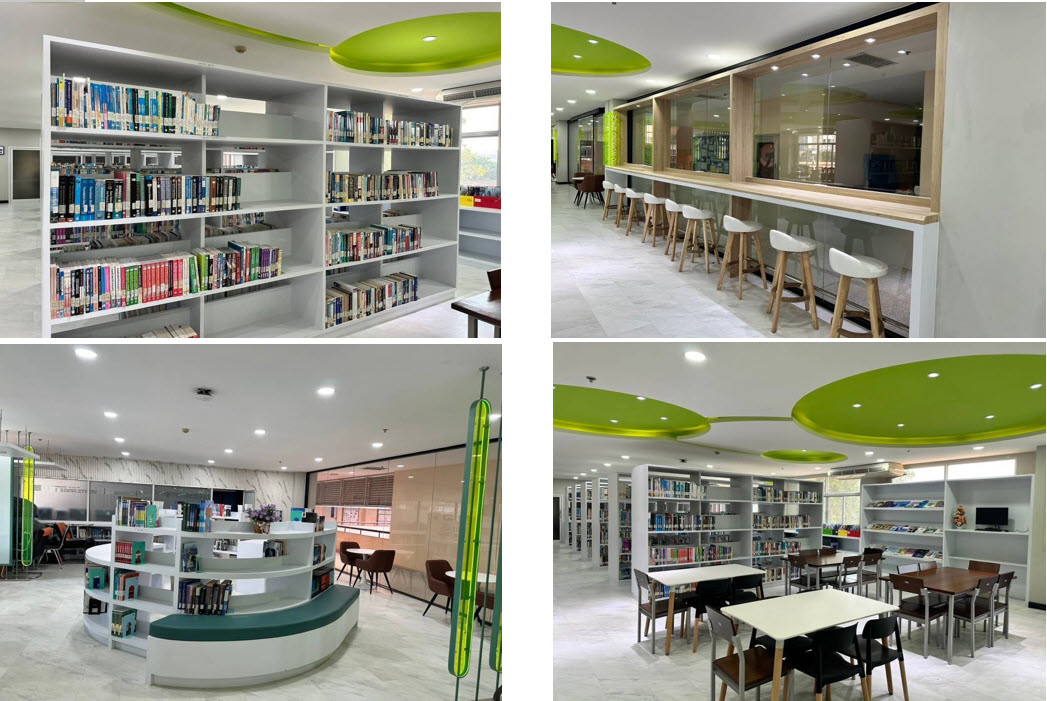
\includegraphics[width=0.8\textwidth]{Pic7.1-3.jpg}\\
\end{center}
ในส่วนของสาขาวิชามีหนังสือเฉพาะทางด้านคณิตศาสตร์  รวมทั้งเล่มโครงงานวิจัยและเล่มรายงานถอดบทเรียนรายวิชาสัมมนาของนักศึกษารุ่นพี่ สำหรับให้บริการนักศึกษา ที่ห้อง ST-1 302 และห้องST-1 908 
\begin{center}
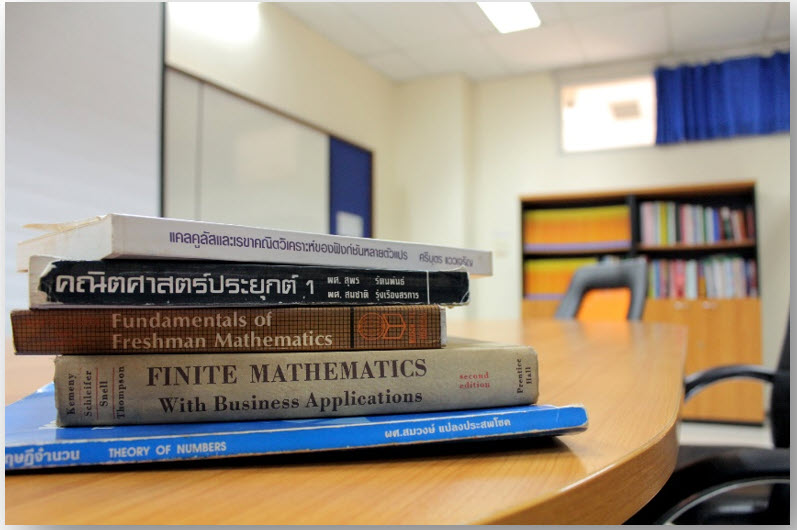
\includegraphics[width=0.8\textwidth]{Pic7.1-4.jpg}\\
\end{center}
\end{enumerate}
\begin{doclist}
	\docitem{ห้องเรียนห้องปฏิบัติการของสาขาวิชา}
	\docitem{ภาพถ่ายห้องสมุดมหาวิทยาลัย ห้องสมุดคณะ ห้องสมุดสาขาวิชา}
\end{doclist}
%%%%%%%%%%%%%%%%%%%% 7.2 %%%%%%%%%%%%%%%
\subcriteria{The laboratories and equipment are shown to be up-to-date, readily available, and effectively deployed.}

สาขาวิชาคณิตศาสตร์ประยุกต์มีห้องปฏิบัติการคอมพิวเตอร์ในความรับผิดชอบจำนวน 1 ห้อง ได้แก่ ห้องปฏิบัติการ ST-1 905 ความจุ 30 ที่นั่ง สำหรับให้บริการกับนักศึกษาที่เรียนในรายวิชาชีพ ของหลักสูตรฯ และรายวิชาชีพบางรายวิชาของหลักสูตรอื่นภายในคณะฯ ในห้องปฏิบัติการมีการลงมีโปรแกรมสำเร็จรูปที่จำเป็นสำหรับนักศึกษาสาขาวิชาคณิตศาสตร์ประยุกต์ เช่น MINITAB  SPSS โปรแกรมฟรี ที่เป็น open source เช่น โปรแกรม R  โปรแกรม Wx Maxima และ โปรแกรม Python เป็นต้น และมีการ update version ของโปรแกรมคอมพิวเตอร์อยู่เสมอเพื่อประโยชน์ในการใช้งานของอาจารย์และนักศึกษา โดยสาขาวิชามีเจ้าหน้าที่ห้องปฏิบัติการคอมพิวเตอร์ 1 คน ที่ดูแลและอำนวยความสะดวกให้กับนักศึกษาและอาจารย์ 

นอกจากนี้สาขาวิชาคณิตศาสตร์ประยุกต์ได้รับจัดสรรงบประมาณในการจัดซื้อวัสดุการศึกษาในปีการศึกษา 2566 จำนวน 43,500 บาท สำหรับนักศึกษาวิชาชีพในหลักสูตร เพื่อใช้ในการจัดซื้อวัสดุในการจัดการเรียนการสอนและปรับปรุงวัสดุต่างๆ ในห้องปฏิบัติการให้มีความพร้อมในการจัดการเรียนการสอนอยู่เสมอ



\begin{doclist}
	\docitem{ห้องปฏิบัติการของสาขาวิชา}
\end{doclist}

%%%%%%%%%%%%% 7.3 %%%%%%%%%%%%%
\subcriteria{A digital library is shown to be set-up, in keeping with progress in information and communication technology.}

หลักสูตรวิทยาศาสตรบัณฑิต สาขาวิชาคณิตศาสตร์ประยุกต์ ใช้ทรัพยากรด้านห้องสมุดดิจิทัลของ
มหาวิทยาลัย ซึ่งรับผิดชอบโดย สำนักวิทยบริการและเทคโนโลยีสารสนเทศ (สวส.) ที่ให้บริการฐานข้อมูลหนังสืออิเล็กทรอนิกส์ (e-Book) สำหรับนักศึกษา คณาจารย์ นักวิจัย และบุคลากรของมหาวิทยาลัยเทคโนโลยีราชมงคลธัญบุรี เพื่อการสืบค้นและการใช้งานฐานข้อมูลหนังสืออิเล็กทรอนิกส์สามารถเข้าถึงข้อมูลสารสนเทศตลอดจนเอกสารฉบับเต็มได้ ซึ่งบริการต่าง ๆ ประกอบไปด้วย
\begin{enumerate}
\item ฐานข้อมูลอิเล็กทรอนิกส์ ฐานข้อมูลอิเล็กทรอนิกส์เพื่อการสืบค้น เป็นการให้บริการฐานข้อมูล
อิเล็กทรอนิกส์ออนไลน์ในต่างประเทศและภายในประเทศไทย เพื่อให้บริการแก่นักศึกษา อาจารย์ บุคลากร และนักวิจัยของมหาวิทยาลัย ให้สามารถใช้ทรัพยากรและเข้าถึงข้อมูลสารสนเทศเอกสารฉบับเต็มได้สะดวก รวดเร็ว ผ่านเครือข่ายสารสนเทศของมหาวิทยาลัยฯ  ซึ่งประกอบไปด้วย 3 ส่วนคือ \\[0.2cm]
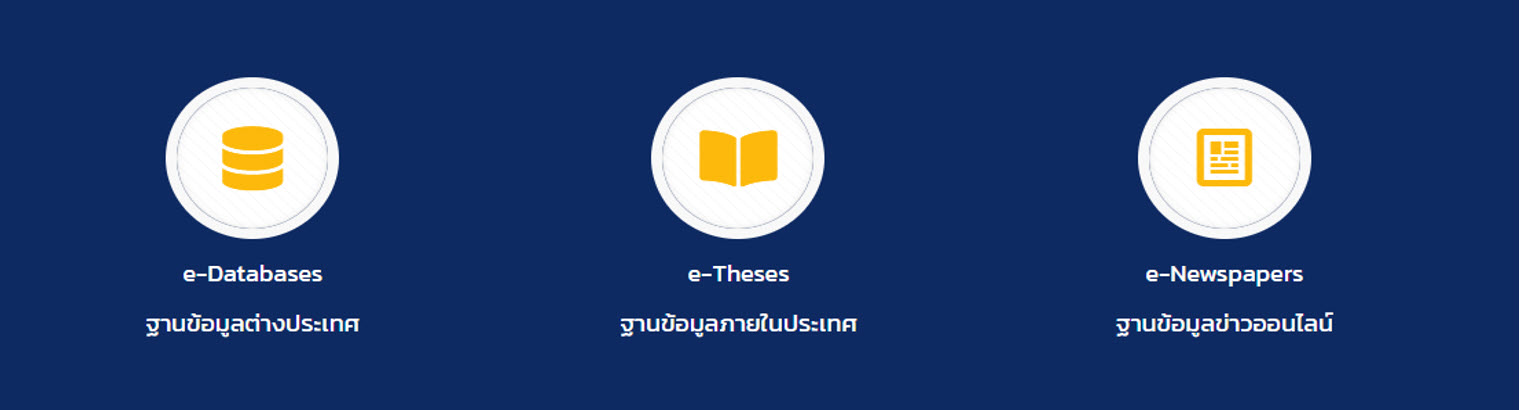
\includegraphics[width=0.9\textwidth]{Pic7.3-1.jpg}
\begin{itemize}
	\item e-Databases เป็นฐานข้อมูลอิเล็กทรอนิกส์ออนไลน์ต่างประเทศ สนับสนุนโดย สำนัก
	ปลัดกระทรวงการอุดมศึกษา วิทยาศาสตร์ วิจัยและนวัตกรรม (อว.) ซึ่งฐานข้อมูลที่ให้บริการประกอบด้วย ฐานข้อมูลอ้างอิง (Reference Database) จำนวน 9 ฐานข้อมูล ที่เกี่ยวกับฐานข้อมูลวารสารอิเล็กทรอนิกส์ในสาขาวิชาต่าง ๆ รวมถึงฐานข้อมูลออนไลน์ที่บอกรับโดย สำนักวิทยบริการและเทคโนโลยีสารนิเทศ มทร.ธัญบุรี
	\\[0.2cm]
	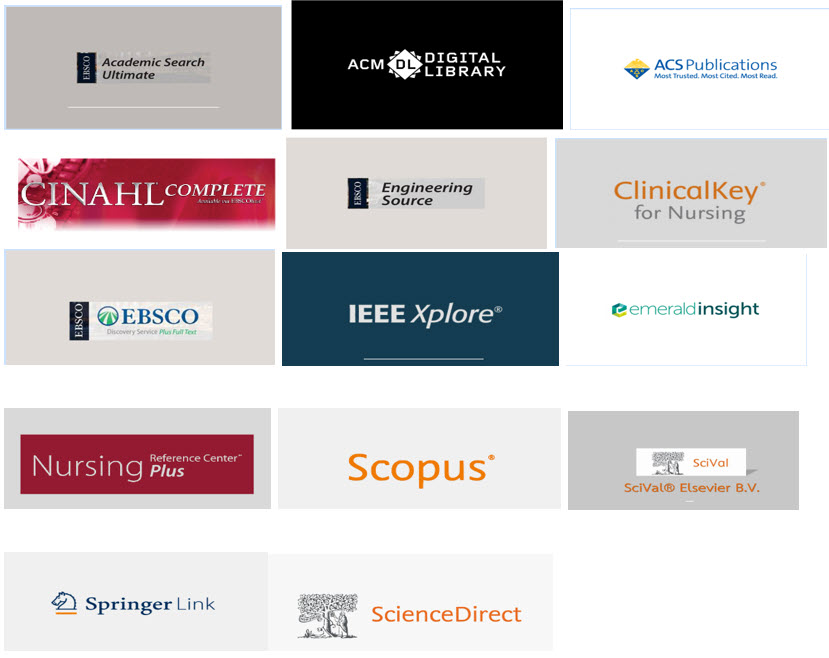
\includegraphics[width=0.8\textwidth]{Pic7.3-2.jpg}\\
	\item e-Theses เป็นการให้บริการฐานข้อมูลอิเล็กทรอนิกส์ออนไลน์ภายในประเทศ สำหรับสืบค้น
	ผลงานทางวิชาการของมหาวิทยาลัยภายในประเทศไทย และผลงานทางวิชาการของมหาวิทยาลัยเทคโนโลยีราชมงคลธัญบุรี ซึ่งประกอบด้วย งานวิจัย วิทยานิพนธ์ บทความวิชาการ และเอกสารเผยแพร่อื่น ๆ
	\item e-Newspapers ฐานข้อมูลข่าวออนไลน์ เป็นบริการกฤตภาคข่าวออนไลน์ (Online News 
	Clipping) โดยการตัดข่าวที่น่าสนใจจากหน้าหนังสือพิมพ์ต่างๆ พร้อมกับระบุแหล่งที่มาของหนังสือพิมพ์ เช่น ฉบับที่ วันที่ข่าว หัวข่าว เนื้อหาข่าว รูปภาพประกอบ (ถ้ามี) เป็นต้น โดยรวบรวมและจัดเก็บไว้ให้บริการผ่านฐานมูลออนไลน์
\end{itemize}
\item บริการด้านภาษา เป็นการบริการโปรแกรมสำหรับฝึกทักษะทางด้านภาษา ทั้งทักษะภาษาอังกฤษ 
ภาษาจีน รวมถึงภาษาอาเซียน ซึ่งแต่ละโปรแกรมมุ่งเน้นให้ผู้รับบริการมีการพัฒนาทักษะการฟัง การพูด การอ่าน และคำศัพท์ เพื่อประยุกต์ใช้ในชีวิตประจำวัน การเรียนและการทำงานได้
\\
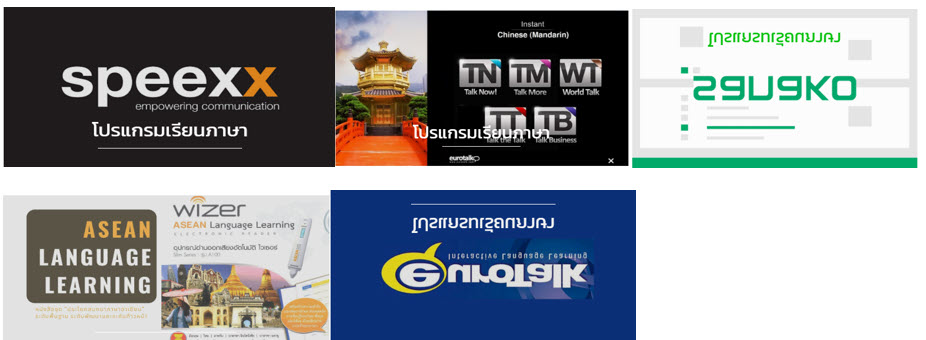
\includegraphics[width=0.9\textwidth]{Pic7.3-3.jpg}\\
%{\bf ภาพที่ 7.3-3} บริการด้านภาษา
\item มีระบบ DLearn@RMUTT เป็นระบบจัดการเรียนการสอนในระบบออนไลน์ให้มีบรรยากาศ
เหมือนการเรียนในห้องเรียน หรือเรียกว่า LMS (Learning Management System) นักศึกษา อาจารย์ หรือบุคลากรของมหาวิทยาลัยสามารถใช้งานระบบ RMUTT D-Learn เพื่อจัดการเรียนการสอนได้ โดยอาจารย์สามารถจัดการรายวิชาของตนเองได้ เช่น การกำหนดบทเรียนและสื่อการสอน การกำหนดงานที่ได้รับมอบหมาย การทำแบบทดสอบ เป็นต้น รวมถึงนักศึกษาสามารถเข้าเรียนออนไลน์ได้ตลอดเวลา ซึ่งเหมาะกับการเรียนแบบ Flipped Classroom รวมถึงทำงานร่วมกับเครื่องมือติดต่อสื่อสารสำหรับประชุมออนไลน์ ระหว่างอาจารย์และนักศึกษาได้
\item ให้บริการการตั้งค่าการเชื่อมต่อ เครือข่ายมหาวิทยาลัยฯ (VPN) เพื่อ Remote Desktop 
Connection, ERP หรือ การสืบค้นงานวิจัย  VPN-RMUTT เป็นระบบเครือข่ายในมหาวิทยาลัยฯ ที่อนุญาตให้คณาจารย์ บุคลากรและนักศึกษาของมหาวิทยาลัย ที่อยู่นอกสถานที่สามารถเชื่อมต่อเข้ามาในเครือข่ายส่วนตัวของมหาวิทยาลัยฯ เสมือนว่าอยู่ในเครือข่ายเดียวกับมหาวิทยาลัยฯ เพื่อให้ง่ายต่อการทำงานต่างๆ ไม่ว่าจะเป็นการเข้าใช้ Remote Desktop Connection , ERP , การสืบค้นงานวิจัย โดยการเข้าใช้งานต้องมี ชื่อผู้ใช้และรหัสผ่าน ซึ่งเป็นชุดเดียวกับ การ Login เข้าใช้งานเครือข่ายอินเทอร์เน็ต WiFi ของมหาวิทยาลัย


\end{enumerate}
\begin{doclist}
	\docitem{เว็บไซต์ห้องสมุดมหาวิทยาลัย\newline https://www.library.rmutt.ac.th/language/}
\end{doclist}

%%%%%%%%%%%%% 7.4 %%%%%%%%%%%%%%%%
\subcriteria{The information technology systems are shown to be set up to meet the needs of staff and students.}

หลักสูตรวิทยาศาสตรบัณฑิตสาขาวิชาคณิตศาสตร์ประยุกต์ ใช้ระบบเทคโนโลยีสารสนเทศที่ตอบสนองความต้องการของบุคลากรและนักศึกษา 2 ส่วน ด้วยกัน คือระบบเทคโนโลยีสารสนเทศของมหาวิทยาลัย และระบบเทคโนโลยีสารสนเทศที่คณะ ฯ พัฒนาขึ้นเอง
\begin{enumerate}
\item ระบบสารสนเทศของมหาวิทยาลัย\\
\underline{ระบบสารสนเทศที่สนับสนุนด้านการเรียนการสอน}
\begin{itemize} 
\item ระบบบริการการศึกษา (https://oreg.rmutt.ac.th/?page\_id=14908)\\ เป็นระบบสารสนเทศที่มีบทบาทอย่างมากสำหรับนักศึกษา อาจารย์ที่ปรึกษา เพราะเป็นระบบที่นักศึกษาสามารถเข้ามาติดตามข่าวสารต่าง ๆ ค้นหารายวิชาเรียน ลงทะเบียนเรียนออนไลน์ ตรวจสอบผลการลงทะเบียนเรียนและพิมพ์ใบแจ้งยอดชาระเงิน ตรวจสอบตารางเรียนและตารางสอบ ตลอดจนตรวจสอบผลการเรียนของตนเอง การยื่นคำร้องออนไลน์ การถอนรายวิชาออนไลน์ และในส่วนของอาจารย์ที่ปรึกษา ระบบ OREG อานวยความสะดวกในการติดตามความก้าวหน้าและผลการเรียนของนักศึกษาเพื่อที่ช่วยให้อาจารย์ที่ปรึกษาวางแผน ให้คำแนะนำ ตลอดจนช่วยแก้ไขปัญหาให้กับนักศึกษา\\[0.2cm]
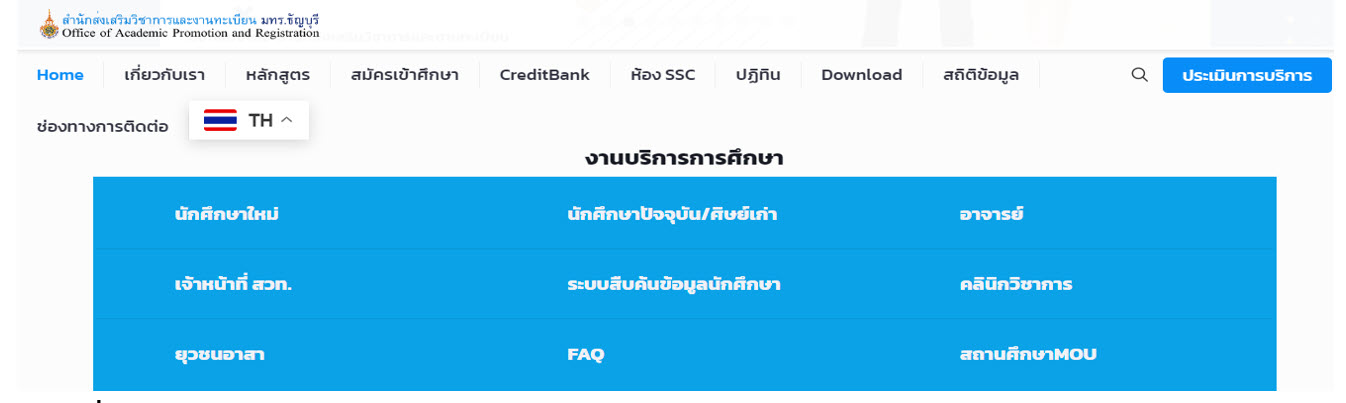
\includegraphics[width=0.8\textwidth]{Pic7.4-1.jpg}\\[0.2cm]
%\indent { \bf ภาพที่ 7.4-1} ระบบบริการการศึกษา
\item ระบบรับสมัครนักศึกษาออนไลน์ \\เป็นระบบที่อำนวยความสะดวกให้นักเรียน มัธยมศึกษาตอนปลาย หรือผู้ต้องการเข้าศึกษาต่อสามารถดำเนินการสมัครเรียนและยื่นเอกสารได้จากทุกที่ทุกเวลา ซึ่งในระบบนี้ผู้สมัครเรียนสามารถตรวจสอบผลการสอบ ดำเนินการรายงานตัว ตรวจสอบสถานะการรายงานตัว พิมพ์ใบชำระเงิน\\[0.2cm]
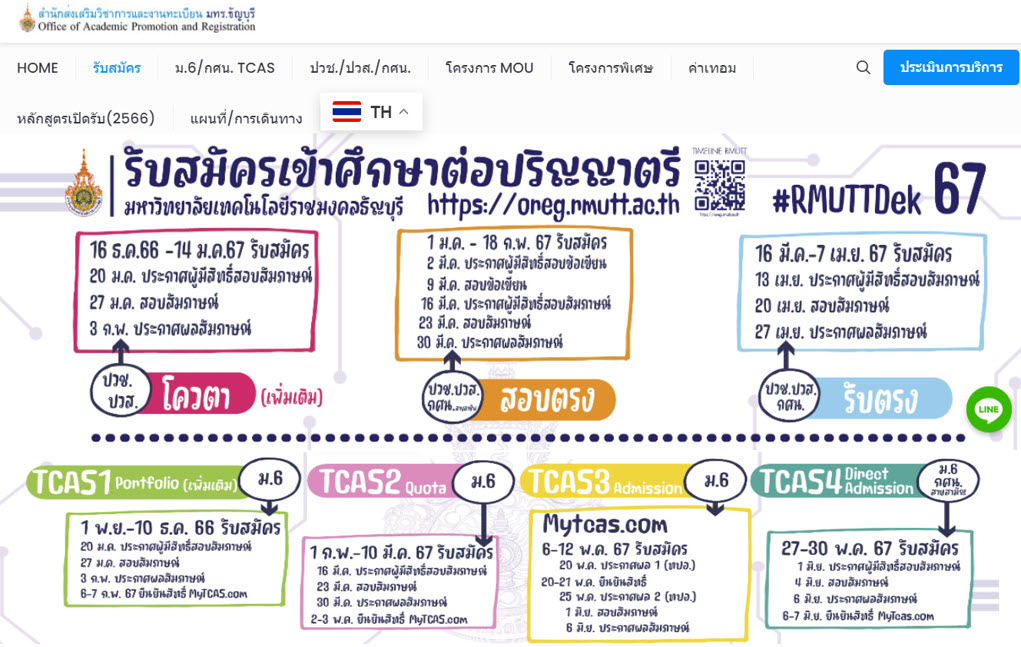
\includegraphics[width=0.8\textwidth]{Pic7.4-2.jpg}\\[0.2cm]
%\indent { \bf ภาพที่ 7.4-2} ระบบรับสมัครนักศึกษาออนไลน์
\end{itemize}
\underline{ระบบสารสนเทศสนับสนุนด้านการวิจัย}
\begin{itemize}
\item ระบบข้อมูลสารสนเทศวิจัยและนวัตกรรม มทร.ธัญบุรี ที่ช่วยในการติดตามและบริการจัดการงานวิจัยทั้งหมดจำนวน  3,440 โครงการ ทั้งงานวิจัยที่เป็นงบประมาณรายจ่าย งบประมาณรายได้ งบประมาณกองทุนส่งเสริมงานวิจัย และงบประมาณส่วนตัว ของทุกคณะ/หน่วยงาน ในมหาวิทยาลัย\\[0.2cm]
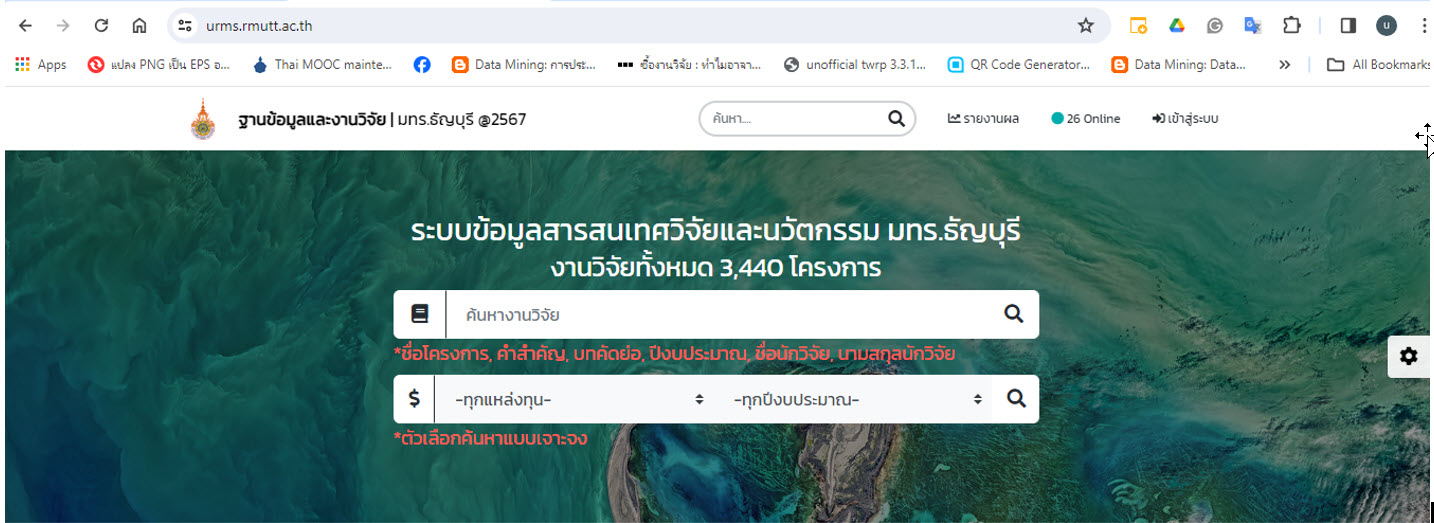
\includegraphics[width=0.7\textwidth]{Pic7.4-3.jpg}\\[0.2cm]
%\indent { \bf ภาพที่ 7.4-3} ระบบข้อมูลสารสนเทศวิจัยและนวัตกรรม มทร.ธัญบุรี
\end{itemize}
\underline{ระบบสารสนเทศที่เพื่อการบริหารจัดการ}
\begin{itemize}
	\item ระบบบุคลากรออนไลน์ (hr-online) 
	บุคลากรสามารถเข้าดูข้อมูลบุคลากรรายบุคคลประวัติการลาของบุคลากร ใบแจ้งเงินเดือน ปฏิทินการลงเวลา แจ้งผลการเลื่อนเงินเดือน เครื่องราชอิสริยาภรณ์ พิมพ์คำร้องขอแก้ไขข้อมูลประวัติส่วนตัว แสดงความคิดเห็น และสอบถามข้อมูล (ถาม-ตอบ) กราฟแสดงผลการประเมินเลื่อนเงินเดือนย้อนหลัง 5 ปี
	\item ระบบสำนักงานอิเล็กทรอนิกส์ (e-office) การบริหารจัดการเอกสารเข้า-ออก จดหมาย
	อิเล็กทรอนิกส์ การจัดเก็บเอกสาร แก้ไขเอกสาร งานเอกสารทางด้านบัญชี และการใช้ประโยชน์อื่น ๆ อีกมากมาย โดยอำนวยความสะดวกในเรื่องการลดขั้นตอน ลดระยะเวลา ลดการใช้ทรัพยากรกระดาษ (paperless) และอำนวยความสะดวกในการบริหารจัดการ การรับ-ส่งข้อมูลข่าวสาร มีการจัดเก็บเอกสารในลักษณะไฟล์ดิจิทัลอย่างเป็นระบบ มีความสะดวกรวดเร็ว และสามารถเข้าถึงและค้นหาข้อมูลได้ง่าย แม้ว่าผู้ปฏิบัติงานจะไม่อยู่ในสำนักงานก็สามารถเข้าถึงข้อมูลได้
	\item ระบบประชุมอิเล็กทรอนิกส์ (e-Meeting)
	\item ระบบจองห้องออนไลน์
\end{itemize}
\item ระบบสารสนเทศที่พัฒนาขึ้นเองโดยคณะวิทยาศาสตร์และเทคโนโลยี 
\begin{itemize}
	\item ระบบบริหารข้อมูลงานวิจัยและงานบริการวิชาการคณะวิทยาศาสตร์และเทคโนโลยี\\ เพื่อบริหารจัดการระบบบริหารข้อมูลงานวิจัยและงานบริการวิชาการ เพื่อเป็นแหล่งรวบรวมข้อมูลผลงานทางวิชาการ งานวิจัยตีพิมพ์ โครงการวิจัย งานวิจัยที่นำไปใช้ประโยชน์ นวัตกรรม ช่วยในการการค้นคว้าอ้างอิง การรายงานผล ตอบโจทย์ยุทธศาสตร์ด้านงานวิจัยและบริการวิชาการของคณะฯ และมหาวิทยาลัยฯ
	\item 	ระบบจัดการข้อมูลการประเมินบุคลากรคณะวิทยาศาสตร์และเทคโนโลยีออนไลน์\\ เพื่อช่วยบริหารจัดการเกี่ยวกับการประเมินผลการปฏิบัติราชการของบุคลากรสายวิชาการของคณะในทุกกลุ่ม ประกอบไปด้วย 
	1) พนักงานมหาวิทยาลัยวุฒิปริญญาเอก 2) พนักงานมหาวิทยาลัยวุฒิปริญญาโท 3) ข้าราชการพลเรือน 4) ข้าราชการ (ที่เป็นผู้บริหาร) และ 5) พนักงานมหาวิทยาลัยวุฒิปริญญาเอก (ที่เป็นผู้บริหาร) 
\end{itemize}
\end{enumerate}

\begin{doclist}
	\docitem{ระบบสารสนเทศของมหาวิทยาลัย}
	\docitem{ระบบสารสนเทศที่พัฒนาขึ้นเองโดยคณะวิทยาศาสตร์และเทคโนโลยี}
\end{doclist}
%%%%%%%%%%% 7.5 %%%%%%%%%%%%%%%%%%%%%%%%%%
\subcriteria{The university is shown to provide a highly accessible computer and network infrastructure that enables the campus community to fully exploit information technology for teaching, research, service, and administration.}

หลักสูตรวิทยาศาสตรบัณฑิต สาขาวิชาคณิตศาสตร์ประยุกต์ ใช้ระบบโครงสร้างพื้นฐานด้านคอมพิวเตอร์และระบบเครือข่ายเทคโนโลยีสารสนเทศที่มีการจัดเตรียมและให้บริการโดยสำนักวิทยบริการและเทคโนโลยีสารสนเทศ (สวส.) โดยระบบดังกล่าวมีความทันสมัย เพียงพอ และพร้อมใช้ ตรงกับความต้องการของทั้งในด้านการเรียนการสอน การวิจัย การบริการวิชาการ และการบริหารจัดการ ซึ่งประกอบไปด้วย
\begin{enumerate}
	\item การใช้บริการเครือข่ายไร้สาย (WIFI-RMUTT) มหาวิทยาลัยเทคโนโลยีราชมงคลธัญบุรี ทางสำนักวิทยบริการและเทคโนโลยีสารสนเทศได้ให้บริการครอบคลุมทั่วทุกจุดใน มทร.ธัญบุรี เช่น
	\begin{itemize}[label=-]
	\item  บริเวณสำนักวิทยบริการและเทคโนโลยีสารสนเทศ\newline(อาคาร ICT, Training, iWork@RT, Library )
	\item อาคารเรียนตามคณะต่าง ๆ
	\item บ้านพักสวัสดิการ ข้าราชการ มทร.ธัญบุรี
	\item หอพักสวัสดิการนักศึกษา มทร.ธัญบุรี
	\item อาคารเรียนรวมและปฏิบัติการ
\end{itemize}
\hspace*{1cm}บุคลากรสามารถเข้าใช้บริการ Wifi@RMUTT ได้โดยใช้ Username : ประกอบด้วย ชื่อ
	ภาษาอังกฤษ ตามด้วยสัญลักษณ์ (\_) และตามด้วยอักษรตัวแรกของนามสกุลภาษาอังกฤษ เช่น ชื่อ Somsak Rmutt ในการกำหนด username จะกำหนดเป็น somsak\_r (ในกรณีนามสกุลตัวแรกซ้ำจะตามด้วยนามสกุลตัวแรกและตัวที่ 2 ของนามสกุล) Password : กำหนดเป็นตัวเลข 6 หลักท้ายจากรหัสบัตรประชาชน
	(โดยบุคลากรสามารถเปลี่ยน Password ได้ด้วยตนเองในภายหลัง) \\[0.2cm]
\hspace*{1cm}นักศึกษาสามารถเข้าใช้บริการ Wifi@RMUTT ได้โดยใช้ Username :  รหัสนักศึกษา 13 หลักโดยไม่ต้องใส่ขีด (-) Password : กำหนดเป็นตัวเลข 6 หลักท้ายจากรหัสบัตรประชาชน
(โดยนักศึกษาสามารถเปลี่ยน Password ได้ด้วยตนเองในภายหลัง)\\[0.2cm]
\hspace*{1cm}ในส่วนของคณะวิทยาศาสตร์และเทคโนโลยีมี 2 อาคารเรียน คือ อาคารเฉลิมพระเกียรติ ๖ รอบพระชนมพรรษา (อาคาร 9 ชั้น) และอาคารสถาบันวิจัยเคมี (อาคาร 4 ชั้น) โดยทุกชั้นของแต่ละอาคารมีจุดเชื่อมต่อสัญญาณ Wifi ทุกชั้น ทำให้สามารถใช้งานได้อย่างไม่ติดขัด \\[0.2cm]
\hspace*{1cm}นอกจากนี้ยังมีการให้บริการการใช้งาน ระบบ Backoffice กรณีที่ไม่ได้ตั้งค่า VPN สามารถตั้งค่า VPN ได้ที่ http://www.ict.rmutt.ac.th/?p=2384  หรือนำเครื่องคอมพิวเตอร์ส่วนบุคคล (Notebook) มาให้เจ้าหน้าที่ที่ สวส. ดำเนินการตั้งค่าระบบ VPN โดยทางสำนักวิทยบริการฯ มีแนวทางจะให้ครอบคลุมทั่วทุกจุดใน มทร.ธัญบุรี ภายในอนาคตเร็ว ๆ นี้
\item 	ในส่วนของคณะมีห้องปฏิบัติคอมพิวเตอร์จำนวน  16  ห้อง รวมจำนวนเครื่องคอมพิวเตอร์ที่ให้บริการนักศึกษา จำนวน 522 เครื่อง โดยมีรายละเอียดดังตาราง 
\begin{center}
%\begin{table}[]
	\begin{tabular}{|c|c|c|c|c|}
		\hline
		\textbf{ลำดับที่} & \textbf{สาขาวิชา}                                                                                                         & \textbf{ชั้น} & \textbf{ห้อง} & \textbf{จำนวนเครื่อง} \\ \hline
		1                 & -                                                                                                                         & 4             & IT\&SCI       & 20                    \\ \hline
		2                 & สาขาวิชาฟิสิกส์                                                                                                           & 7             & ST1-710       & 37                    \\ \hline
		3                 & \multirow{10}{*}{\begin{tabular}[c]{@{}c@{}}สาขาวิชาวิทยาการคอมพิวเตอร์ และ \\ สาขาวิชาเทคโนโลยีคอมพิวเตอร์\end{tabular}} & 8             & ST1-804       & 30                    \\ \cline{1-1} \cline{3-5} 
		4                 &                                                                                                                           & 8             & ST1-805       & 31                    \\ \cline{1-1} \cline{3-5} 
		5                 &                                                                                                                           & 8             & ST1-806       & 31                    \\ \cline{1-1} \cline{3-5} 
		6                 &                                                                                                                           & 8             & ST1-807       & 37                    \\ \cline{1-1} \cline{3-5} 
		7                 &                                                                                                                           & 8             & ST1-809       & 61                    \\ \cline{1-1} \cline{3-5} 
		8                 &                                                                                                                           & 8             & ST1-810       & 30                    \\ \cline{1-1} \cline{3-5} 
		9                 &                                                                                                                           & 8             & ST1-811       & 30                    \\ \cline{1-1} \cline{3-5} 
		10                &                                                                                                                           & 8             & ST1-812       & 31                    \\ \cline{1-1} \cline{3-5} 
		11                &                                                                                                                           & 8             & ST1-813       & 30                    \\ \cline{1-1} \cline{3-5} 
		12                &                                                                                                                           & 8             & ST1-814       & 31                    \\ \hline
		13                & \multirow{4}{*}{\begin{tabular}[c]{@{}c@{}}สาขาวิชาคณิตศาสตร์ และ \\ สาขาวิชาสถิติประยุกต์\end{tabular}}                  & 9             & ST1-904       & 32                    \\ \cline{1-1} \cline{3-5} 
		14                &                                                                                                                           & 9             & ST1-905       & 30                    \\ \cline{1-1} \cline{3-5} 
		15                &                                                                                                                           & 9             & ST1-912       & 36                    \\ \cline{1-1} \cline{3-5} 
		16                &                                                                                                                           & 9             & ST1-914       & 25                    \\ \hline
	\end{tabular}
%\end{table}
\end{center}
%\includegraphics[width=0.85\textwidth]{Table 7.5-1.jpg}
\item สำนักวิทยบริการฯ มีบริการ IT zone ณ อาคารวิทยบริการ จัดพื้นที่ให้ผู้ใช้บริการสามารถใช้คอมพิวเตอร์สำหรับค้นหาข้อมูลทางวิชาการ โปรแกรมการทำงาน เรียนออนไลน์ และนันทนาการ  ผู้ใช้บริการสามารถใช้บริการได้โดยต้องมี Username และ Password WiFi-RMUTT  มีบริการเครื่องคอมพิวเตอร์ สำหรับค้นหาข้อมูลทางวิชาการ โปรแกรมการทำงาน เรียนออนไลน์ และนันทนาการ  รวมทั้งหมดจำนวน 84 เครื่อง  เครื่องคอมพิวเตอร์รองรับการสั่ง พิมพ์เอกสารออนไลน์ ได้จำนวน 64 เครื่อง
\item สำนักวิทยบริการฯ มีการพัฒนาระบบสมุดบันทึกกิจกรรม (Activity RMUTT) สำหรับนักศึกษา
\item สำนักวิทยบริการฯ ให้บริการจองห้อง ประกอบไปด้วย อาคารเรียนรวมและปฏิบัติการ (Central Building)  ห้อง Discussion Room 4-15 ที่นั่ง ห้องปฏิบัติการ Computer 40-80 ที่นั่ง  ห้อง Smart Classroom ห้อง Classroom 40 - 120 ที่นั่ง  ห้องประชุม/สัมมนา 100 ที่นั่ง
\item สำนักวิทยบริการ ฯ ให้บริการระบบห้องเรียนออนไลน์ D-Learn@RMUTT สำหรับอาจารย์ผู้สอนเพื่อจัดการเรียนการสอนในระบบออนไลน์ให้มีบรรยากาศเหมือนการเรียนในห้องเรียน โดยนักศึกษา อาจารย์ หรือบุคลากรของมหาวิทยาลัยที่สนใจสามารถใช้งานระบบ D-Learn@RMUTT เพื่อจัดการเรียนการสอน อาจารย์สามารถจัดการรายวิชาของตนเองได้ เช่น การกำหนดบทเรียนและสื่อการสอน การกำหนดงานมอบหมาย การทำแบบทดสอบ เป็นต้น รวมถึงนักศึกษาสามารถเข้าเรียนออนไลน์ได้ตลอดเวลา ซึ่งเหมาะกับการเรียนแบบ Flipped Classroom รวมถึงทำงานร่วมกับเครื่องมือติดต่อสื่อสารสำหรับประชุมออนไลน์ และการจัดการเรียนการสอนออนไลน์ ผ่านระบบ MS-Teams
\end{enumerate}

\begin{doclist}
	\docitem{ข้อมูลของโครงสร้างพื้นฐานด้านคอมพิวเตอร์และเครือข่ายพื้นฐานที่จัดหาโดยคณะและมหาวิทยาลัย}
\end{doclist}


%%%%%%%%%%% 7.6 %%%%%%%%%%%%%%%%%%%%%%%%%%
\subcriteria{The environmental, health, and safety standards and access for people with special needs are shown to be defined and implemented.}

นักศึกษาของหลักสูตรส่วนใหญ่เรียนในอาคารเรียน อาคารเฉลิมพระเกียรติ ๖ รอบพระชนมพรรษา คณะวิทยาศาสตร์และเทคโนโลยี 9 ชั้น  (ห้องเรียนและห้องปฏิบัติการอยู่บริเวณชั้น 9) เป็นส่วนใหญ่  เนื่องจากเป็นตึกสูงดังนั้นองค์ประกอบด้านความปลอดภัยที่ต้องมีคือ ข้อกำหนดด้านความปลอดภัยในอาคารสูง โดยมีกฎหมายที่เกี่ยวข้องคือ
กฎกระทรวงฉบับที่ 33 (พ.ศ.2535) ฉบับที่ 47 (พ.ศ.2540) ฉบับที่ 48 (พ.ศ.2540) และฉบับที่ 50 (พ.ศ.2540) ออกตามความในพระราชบัญญัติควบคุมอาคาร พ.ศ.2522

{\bf ด้านความปลอดภัย}

การดูแลระบบไฟฟ้าและดับเพลิง เป็นหน้าที่ของงานอาคารสถานที่คณะ มีการจัดเตรียมอุปกรณ์ดับเพลิงที่พร้อมใช้งานในทุกชั้นของอาคาร มีการตรวจสอบอุปกรณ์ถังดับเพลิงสม่ำเสมอ ปีการศึกษาละ 1 ครั้งและมีการจัดการฝึกซ้อมอพยพหนีไฟ ปีการศึกษาละ 1 ครั้ง

ในทุก ๆ ห้องเรียนห้องปฏิบัติการ จะมีระบบรักษาความปลอดภัย ได้แก่
\begin{enumerate}
	\item มีระบบ smoke detector หากพบกลุ่มควันภายในห้องจะมีการแจ้งเตือนไปที่ห้องของเจ้าหน้าที่อาคารสถานที่ของคณะ
	\item มีระบบหัวดับเพลิงติดอยู่บนฝ้าเพดานเมื่อเจอความร้อนจะแตกและปล่อยน้ำในท่อออกมาเพื่อระงับการเกิดเพลิงไหม้
	\item มีตู้ควบคุมระบบไฟฟ้าเพื่อตัดไฟเมื่อเกิดเพลิงไหม้
\end{enumerate}

นอกจากนั้นยังมีการออกกฎข้อปฏิบัติในการใช้ห้องปฏิบัติการคอมพิวเตอร์ โดยมีป้ายเตือนนักศึกษา หลังเลิกใช้เครื่องคอมพิวเตอร์ในห้องปฏิบัติการควรปิดเครื่องคอมพิวเตอร์ให้เรียบร้อยก่อนออกจากห้อง เพื่อป้องกันปัญหาด้านความร้อนของอุปกรณ์คอมพิวเตอร์

{\bf ด้านสุขภาพ}

ในแต่ละปีจะมีการตรวจสุขภาพประจำปีให้กับนักศึกษาและบุคลากรทุกคน และมหาวิทยาลัยได้ดำเนินการจัดทำประกันอุบัติเหตุให้กับนักศึกษาและบุคลากรทุกคนทุกปี ตลอดจนมีการตรวจสารเสพติดในนักศึกษาเพื่อป้องกันปัญหาสารเสพติดในสถานศึกษา มีกิจกรรมอบรมให้ความรู้เกี่ยวกับอันตรายของยาเสพติด/บุหรี่ ซึ่งดำเนินการโดยกองพัฒนานักศึกษา

ด้านสาธารณูปโภคและการรักษาความปลอดภัย
คณะฯ มีการจ้างแม่บ้านในการดูแลทำความสะอาดกำจัดขยะมูลฝอยในหน่วยงานทุกวัน และจัดกิจกรรม 5 ส ภายในหน่วยงานและมีการประกวดกิจกรรม 5 ส ในทุก ๆ ปี ในแต่ละชั้นของตึกมีน้ำดื่มที่สะอาดให้บริการกับนักศึกษา
ในส่วนการเข้าถึงของบุคคลที่มีความต้องการพิเศษ (Access for People with special needs) มีการดำเนินการเช่น จัดให้มีทางลาด ขึ้น ลง อาคาร จัดให้มีลิฟต์หรือทางลาดที่ผู้พิการหรือทุพพลภาพ และคนชรา ใช้ได้  จัดให้มีห้องน้ำสำหรับผู้พิการหรือทุพพลภาพ เป็นต้น


\begin{doclist}
	\docitem{ข้อมูลมาตรฐานด้านความปลอดภัย/สิ่งแวดล้อม }
	\docitem{ข้อมูลมาตรฐานของผู้ที่มีความต้องการพิเศษ }
\end{doclist}

%%%%%%%%%%% 7.7 %%%%%%%%%%%%%%%%%%%%%%%%%%
\subcriteria{The university is shown to provide a physical, social, and psychological environment that is conducive for education, research, and personal well-being.}
\begin{enumerate}
\item {\bf ด้านสิ่งแวดล้อมทางกายภาพ}\\ 
กองอาคารสถานที่ของมหาวิทยาลัย และงานสถานที่คณะ เป็นผู้รับผิดชอบการจัดการอาคารสถานที่ ให้มีความพร้อมใช้ เพียงพอต่อจำนวนนักศึกษา โดยมีการทบทวนการจัดสิ่งอำนวยความสะดวกของนักศึกษาทุกสิ้นปีการศึกษา สิ่งอำนวยความสะดวกด้านสิ่งแวดล้อมทางกายภาพประกอบไปด้วย
\begin{enumerate}[label=(\arabic*), leftmargin=1cm]
\item อาคารเฉลิมพระเกียรติ ๖ รอบพระชนมพรรษา คณะวิทยาศาสตร์และเทคโนโลยี 9 ชั้น  ซึ่งประกอบไป
ด้วยห้องเรียน ห้องปฏิบัติการ และพื้นที่การเรียนรู้ Learning Space สำหรับนักศึกษาในการศึกษาค้นคว้าความรู้ด้วยตนเองและทำวิจัย 
\item ห้องเอนกประสงค์ ชั้น 1 (นลินวิทย์) เพื่อใช้จัดกิจกรรม หรือเวทีการประกวดต่างๆ หรือใช้ซ้อมการแสดง 
\item พื้นที่บริเวณลานปาล์มและชั้น 1 ของคณะที่ปรับทัศนียภาพเป็นลักษณะสวนหย่อม เพื่อใช้พักผ่อนหย่อนใจ 
\item ชั้น 1 อาคารเฉลิมพระเกียรติ ๖ รอบพระชนมพรรษา คณะวิทยาศาสตร์และเทคโนโลยีมีพื้นที่ให้นักศึกษานั่งทำกิจกรรมหรือรอเรียน
\item มีสนามกีฬาบริการให้กับนักศึกษา
\item มีห้องพยาบาล 
\item ที่จอดรถบริเวณรอบคณะ
\item ร้านถ่ายเอกสาร / เครื่องถ่ายเอกสาร 
\item มีรถไฟฟ้ารับส่งภายในพื้นที่ มทร.ธัญบุรี  และสกู๊ตไฟฟ้าพลังงานสะอาด ไม่ต้องเติมน้ำมัน
 รักษาสิ่งแวดล้อม
\end{enumerate}
\item {\bf ด้านสิ่งแวดล้อมทางสังคม}\\ 
กองพัฒนานักศึกษาเป็นผู้รับผิดชอบการจัดชมรม จัดกิจกรรมพัฒนาศักยภาพของนักศึกษาในภาพรวมของมหาวิทยาลัย รวมถึงคณะดำเนินการจัดโครงการพัฒนาศักยภาพของนักศึกษาในภาพรวมของคณะ ตัวอย่างของการจัดหาสิ่งแวดล้อมทางสังคม เช่น 
\begin{enumerate}[label=(\arabic*), leftmargin=1cm]
\item กิจกรรมพิเศษนอกหลักสูตร :  มีการจัดกิจกรรมพิเศษนอกหลักสูตรต่าง ๆ ให้แก่ นักศึกษาสามารถเข้าร่วมกิจกรรม เพื่อเป็นการพัฒนาและเสริมสร้างทักษะด้านต่าง ๆ เช่น พิธีการไหว้ครู โครงการปัจฉิมนิเทศนักศึกษา โครงการรับน้องใหม่ เป็นต้น
\item กิจกรรมชมรม : มีการสนับสนุนการจัดตั้งชมรมแก่นักศึกษา เช่น ชมรม green university 
\item สโมสรนักศึกษา : มีการจัดตั้งกรรมการบริหารสโมสรนักศึกษา ซึ่งมีตัวแทนจากนักศึกษาแต่ละสาขาร่วมกันวางแผนการจัดกิจกรรมที่นักศึกษาสนใจ
\item การจัดหาแหล่งงานทั้งเต็มเวลาและนอกเวลาให้แก่นักศึกษา : กองพัฒนานักศึกษา มหาวิทยาลัย และฝ่ายพัฒนานักศึกษาของคณะมีการจัดหาแหล่งงานทั้งเต็มเวลาและนอกเวลาให้แก่นักศึกษา ผ่านการจัดกิจกรรม JOB Fair RMUTT  Facebook คณะ Facebook มหาวิทยาลัย บอร์ดประชาสัมพันธ์แหล่งงาน เป็นต้น
\end{enumerate}
\item {\bf ด้านจิตใจ }\\
กองพัฒนานักศึกษา มหาวิทยาลัยเทคโนโลยีราชมงคลธัญบุรี เปิดคลินิกกำลังใจ ให้คำปรึกษา พัฒนากำลังใจ วิเคราะห์ สร้างคุณภาพชีวิตที่ดีขึ้นให้กับนักศึกษา โดยมีผู้เชี่ยวชาญและห้องบริการให้บริการการปรึกษาเชิงจิตวิทยา มุ่งส่งเสริมสุขภาวะทางจิตที่ดีแก่นักศึกษา ให้ข้อมูลเผยแพร่องค์ความรู้ทางจิตวิทยา เพื่อส่งเสริมการดำเนินชีวิตให้มีสุขภาวะทางจิตใจที่ดี มีสติรู้เท่าทัน และสามารถจัดการอารมณ์เพื่อใช้ชีวิตอย่างมีความสุข และให้บริการปรึกษาเชิงจิตวิทยาแก่นักศึกษา ทั้งทางโทรศัพท์และการเข้าพบเพื่อให้คำปรึกษาเป็นรายบุคคล 
\item {\bf ด้านเอื้ออาทรอื่น ๆ }\\
กองพัฒนานักศึกษามหาวิทยาลัยและฝ่ายพัฒนานักศึกษาคณะ เป็นผู้รับผิดชอบงานทุนการศึกษา และการให้บริการด้านต่าง ๆ ดังนี้
\begin{enumerate}[label=(\arabic*), leftmargin=1cm]
\item ทุนการศึกษา :\\ทุนการศึกษาของมหาวิทยาลัยแบ่งจัดสรรให้แก่นักศึกษาทุกคณะ/สาขาวิชา และทุนการศึกษาจากบุคคลภายนอก/สถานประกอบการภายนอก เป็นเงินทุนสนับสนุนเพื่อส่งเสริมการศึกษาจากผู้มีจิตศรัทธา หน่วยงานการศึกษา สถานประกอบการภายนอกทั้งในประเทศ และต่างประเทศ
\item ทุนให้กู้ยืมจากรัฐบาล :  \\ได้แก่ กองทุนเงินให้กู้ยืมเพื่อการศึกษา (กยศ.) และกองทุนเงินให้กู้ยืมที่ผูกพันกับรายได้ในอนาคต (กรอ.)
\item ทุนช่วยเหลือในลักษณะทุนให้เปล่า : \\ซึ่งเกิดจากความร่วมมือระหว่างสาขาวิชากับศิษย์เก่า และบุคคลทั่วไป เพื่อสนับสนุนค่าครองชีพแก่นักศึกษาทั้งในรูปแบบของตัวเงิน รวมไปถึงการจัดหางานที่เหมาะสมเพื่อมีรายได้เพิ่มเติม
\item สวัสดิการด้านต่าง ๆ เพิ่มเติม : \\การเบิกค่าสินไหมทดแทนเมื่อนักศึกษาประสบอุบัติเหตุ การขอผ่อนผันการเข้ารับราชการทหารกองประจำการ การศึกษาต่อนักศึกษาวิชาทหาร
\end{enumerate}
\end{enumerate}

\begin{doclist}
	\docitem{ข้อมูลการจัดสภาพแวดล้อมเพื่อให้เอื้อต่อสภาพแวดล้อม สังคม และจิตใจ }
\end{doclist}

%%%%%%%%%%% 7.8 %%%%%%%%%%%%%%%%%%%%%%%%%%
\subcriteria{The competences of the support staff rendering services related to facilities are shown to be identified and evaluated to ensure that their skills remain relevant to stakeholder needs.}
เจ้าหน้าที่สายสนับสนุนที่ให้บริการทางด้านสิ่งอำนวยความสะดวกและโครงสร้างพื้นฐานของคณะวิทยาศาสตร์และเทคโนโลยี ประกอบด้วย
\begin{enumerate}
	\item เจ้าหน้าที่ห้องปฏิบัติการ
	\item เจ้าหน้าที่เทคโนโลยีสารสนเทศ
	\item เจ้าหน้าที่งานห้องสมุด
	\item เจ้าหน้าที่งานอาคารสถานที่
\end{enumerate}

การกำหนดสมรรถนะของเจ้าหน้าที่สายสนับสนุนเป็นไปตามกรอบของคณะและมหาวิทยาลัย  โดยคณะมีการจัดทำคำบรรยายลักษณะงาน  (Job Description) คุณสมบัติเฉพาะตำแหน่ง  (Job Specification) ที่ชัดเจนเกี่ยวข้องกับความสามารถในการให้บริการนักศึกษา

สำหรับเจ้าหน้าที่สายสนับสนุนด้านสิ่งอำนวยความสะดวกและโครงสร้างพื้นฐานของหลักสูตรมี 1 คน
คือเจ้าหน้าที่ประจำห้องปฏิบัติการคอมพิวเตอร์ ซึ่งหลักสูตรกำหนดสมรรถนะของเจ้าหน้าที่ประจำห้องปฏิบัติการดังนี้
\begin{enumerate}
	\item มีความเชี่ยวชาญในการติดตั้งโปรแกรมคอมพิวเตอร์
	\item มีความเชี่ยวชาญในการซ่อมคอมพิวเตอร์
	\item มีความเชี่ยวชาญในการประกอบคอมพิวเตอร์
	\item สามารถให้คำแนะนำเกี่ยวกับการใช้ห้องปฏิบัติการแก่นักศึกษาได้
\end{enumerate}

ในปีการศึกษา 2566 หลักสูตรมีการประเมินความคิดเห็นในการให้บริการด้านสิ่งอำนวยความสะดวกและโครงสร้างพื้นฐานตามสมรรถนะของผู้ให้บริการ โดยใช้ระบบการประเมินที่ทางคณะฯ เป็นผู้จัดทำขึ้น เป็นการประเมินในรูปแบบออนไลน์ผ่าน Google Form โดยมีผลการการประเมินดังตาราง
ตาราง \ref{Table 7.8-1} และ \ref{Table 7.8-2} ซึ่งมีการเกณฑ์การแปลผล ดังนี้
\begin{itemize}
\item ระดับความพึงพอใจเฉลี่ย 1.00 – 1.50 มีความคิดเห็นในระดับน้อยที่สุด
\item ระดับความพึงพอใจเฉลี่ย 1.51 – 2.50 มีความคิดเห็นในระดับน้อย
\item ระดับความพึงพอใจเฉลี่ย 2.51 – 3.50 มีความคิดเห็นในระดับปานกลาง
\item ระดับความพึงพอใจเฉลี่ย 3.51 – 4.50 มีความคิดเห็นในระดับมาก
\item ระดับความพึงพอใจเฉลี่ย 4.51 – 5.00 มีความคิดเห็นในระดับมากที่สุด  
\end{itemize}
%%%%%%%%%%%%%%%%%%% อาจารย์ %%%%%%%%%%%%%%%%
  \begin{longtable}{|>{\raggedright}p{9cm}|c|c|}
	\caption{ผลการประเมินความคิดเห็นของอาจารย์ต่อการให้บริการด้านสิ่งอำนวยความสะดวกและโครงสร้างพื้นฐานตามสมรรถนะของผู้ให้บริการ}	
	\label{Table 7.8-1}\\
	\hline
	\centering{\textbf{รายการ}} & 
	{\boldmath{$\bar{x}$}} & \textbf{SD} \\ \hline
	\endfirsthead
	\caption[]{(ต่อ) ผลการประเมินความคิดเห็นของอาจารย์ต่อการให้บริการด้านสิ่งอำนวยความสะดวกและโครงสร้างพื้นฐานตามสมรรถนะของผู้ให้บริการ}	
	\\
	\hline
	\centering{\textbf{รายการ}} & 	{\boldmath{$\bar{x}$}} & \textbf{SD} \\ \hline
	\endhead
    \hline
		\textbf{เจ้าหน้าที่ห้องปฏิบัติการ}                                                                                                                                            & \textbf{4.53}                            & \textbf{0.83}          \\ \hline
		เจ้าหน้าที่มีความรู้ ความสามารถ เกี่ยวกับเครื่องมือ และ ให้คำแนะนำในการใช้เครื่องมือได้อย่างถูกต้อง                                                                           & 4.50                            & 0.84          \\ \hline
		ความสามารถของเจ้าหน้าที่ในการเตรียมห้องปฏิบัติการ เตรียมอุปกรณ์ ตรวจสอบความเรียบร้อยของอุปกรณ์ให้พร้อมใช้                                                                     & 4.67                            & 0.82          \\ \hline
		ความสมารถของเจ้าหน้าที่ในการให้คำแนะนำ ตอบปัญหา แก้ไขปัญหาในห้องปฏิบัติการ                                                                                                    & 4.50                            & 0.84          \\ \hline
		เจ้าหน้าที่ห้องปฏิบัติการให้บริการด้วยถ้อยคำสุภาพ ยิ้มแย้ม และเป็นมิตร                                                                                                        & 4.67                            & 0.82          \\ \hline
		การติดต่อขอรับบริการของท่านในแต่ละครั้งได้รับการอำนวยความสะดวกเป็นอย่างดี ไม่มีปัญหา                                                                                          & 4.50                            & 0.84          \\ \hline
		ความสะดวกในการยืม - คืน เครื่องมือ อุปกรณ์ การเข้าใช้ห้องปฏิบัติการฯ                                                                                                          & 4.33                            & 0.82          \\ \hline
		\textbf{เจ้าหน้าที่เทคโนโลยีสารสนเทศ}                                                                                                                                         & \textbf{4.53}                            & \textbf{0.83}          \\ \hline
		ความสามารถของเจ้าหน้าที่ในการดูแลระบบเครือข่ายอินเตอร์เน็ตครอบคลุมทั่วถึง                                                                                                     & 4.50                            & 0.84          \\ \hline
		เจ้าหน้าที่สามารถดูแลระบบอินเตอร์เน็ตให้มีความเร็วเหมาะสมกับการใช้งาน                                                                                                         & 4.67                            & 0.82          \\ \hline
		มีระบบสารสนเทศแจ้งข้อมูลข่าวสารที่รวดเร็ว เช่น website, Facebook, Line@                                                                                                       & 4.50                            & 0.84          \\ \hline
		ความสามารถของเจ้าหน้าที่ในการดูแลระบบเครือข่ายอินเตอร์เน็ตให้พร้อมใช้งาน                                                                                                      & 4.50                            & 0.84          \\ \hline
		เจ้าหน้าที่สามารถตอบปัญหา แก้ไขปัญหาหากมีปัญหาเกี่ยวกับระบบเครือข่าย                                                                                                          & 4.50                            & 0.84          \\ \hline
		\textbf{เจ้าหน้าที่ห้องสมุด}                                                                                                                                                  & \textbf{4.57}                            & \textbf{0.83}          \\ \hline
		เจ้าหน้าที่มีความรู้ ความสามารถ เกี่ยวกับทักษะด้านการบริหารจัดการห้องสมุด                                                                                                     & 4.67                            & 0.82          \\ \hline
		ความสามารถของเจ้าหน้าที่ในการจัดบริการสารสนเทศ                                                                                                                                & 4.50                            & 0.84          \\ \hline
		ความสมารถของเจ้าหน้าที่ในการให้คำแนะนำ ตอบปัญหา แก้ไขปัญหา                                                                                                                    & 4.50                            & 0.84          \\ \hline
		เจ้าหน้าที่ห้องสมุดให้บริการด้วยถ้อยคำสุภาพ ยิ้มแย้ม และเป็นมิตร                                                                                                              & 4.50                            & 0.84          \\ \hline
		การติดต่อขอรับบริการของท่านในแต่ละครั้งได้รับการอำนวยความสะดวกเป็นอย่างดี ไม่มีปัญหา                                                                                          & 4.67                            & 0.82          \\ \hline
		ความสะดวกในการยืม - คืน ทรัพยากรห้องสมุด                                                                                                                                      & 4.33                            & 0.82          \\ \hline
		\textbf{เจ้าหน้าที่อาคารสถานที่}                                                                                          & \textbf{4.56} & \textbf{0.83}       \\ \hline
		ความสามารถของเจ้าหน้าที่ในการดูแลอาคารสถานที่ให้มีความสะอาดเรียบร้อย                                                                                                          & 4.67                            & 0.82          \\ \hline
		ความสามารถของเจ้าหน้าที่ในการดูแลอาคารสถานที่ให้มีความปลอดภัย เช่น ทุกชั้นของอาคารต้องจัดให้มีตู้หัวฉีดน้ำดับเพลิงที่ประกอบ ด้วยหัวต่อสายฉีดน้ำดับเพลิงพร้อมสายฉีดน้ำดับเพลิง & 4.67                            & 0.82          \\ \hline
		ความสามารถของเจ้าหน้าที่ในการดูแลและบำรุงรักษาระบบสาธารณูปโภค ให้มีสภาพพร้อมใช้งาน                                                                                            & 4.50                            & 0.84          \\ \hline
		ความสามารถของเจ้าหน้าที่ในการดูแลห้องเรียน ห้องประชุมให้พร้อมใช้งานอยู่เสมอ                                                                                                   & 4.50                            & 0.84          \\ \hline
		ความสามารถของเจ้าหน้าที่ในการดูแลอุปกรณ์โสตทัศนูปกรณ์วัสดุ ครุภัณฑ์ ให้พร้อมใช้งาน                                                                                            & 4.50                            & 0.84          \\ \hline
		ความสามารถของเจ้าหน้าที่ในการแก้ไขปัญหาเกี่ยวกับงานอาคารสถานที่หากมีปัญหาเกี่ยวกับงานอาคารสถานที่ เช่น ระบบไฟฟ้า ประปา                                                        & 4.50                            & 0.84          \\ \hline
		\multicolumn{1}{|r|}{\textbf{ค่าเฉลี่ยรวม}}       & \textbf{4.55}                            & \textbf{0.83}          \\ \hline

\end{longtable}

จากตารางพบว่าความคิดเห็นของอาจารย์ต่อการให้บริการด้านสิ่งอำนวยความสะดวกและโครงสร้างพื้นฐานตามสมรรถนะของผู้ให้บริการในภาพรวมอยู่ในระดับมากที่สุด ($\bar{x}$=4.55 SD=0.83) ความคิดเห็นในทุกประเด็นของการให้บริการอยู่ในระดับมากที่สุดทุกประเด็น 
%%%%%% นักศึกษา %%%%%%%%%%%%%%5
  \begin{longtable}{|>{\raggedright}p{9cm}|c|c|}
	\caption{ผลการประเมินความคิดเห็นของนักศึกษาต่อการให้บริการด้านสิ่งอำนวยความสะดวกและโครงสร้างพื้นฐานตามสมรรถนะของผู้ให้บริการ}	
	\label{Table 7.8-2}\\
	\hline
	\centering{\textbf{การให้บริการและช่วยเหลือผู้เรียน}} & 
		{\boldmath{$\bar{x}$}} & \textbf{SD}  \\ \hline
	\endfirsthead
	\caption[]{(ต่อ) ผลการประเมินความคิดเห็นของนักศึกษาต่อการให้บริการด้านสิ่งอำนวยความสะดวกและโครงสร้างพื้นฐานตามสมรรถนะของผู้ให้บริการ}	
	\\
	\hline
	\centering{\textbf{การให้บริการและช่วยเหลือผู้เรียน}} & 	{\boldmath{$\bar{x}$}} & \textbf{SD} \\ \hline
	\endhead
		\textbf{เจ้าหน้าที่ห้องปฏิบัติการ}                                                                                                                                            & \textbf{4.07}                            & \textbf{0.93}        \\ \hline
		เจ้าหน้าที่มีความรู้ ความสามารถ เกี่ยวกับเครื่องมือ และ ให้คำแนะนำในการใช้เครื่องมือได้อย่างถูกต้อง                                                                           & 4.13                            & 0.94        \\ \hline
		ความสามารถของเจ้าหน้าที่ในการเตรียมห้องปฏิบัติการ เตรียมอุปกรณ์ ตรวจสอบความเรียบร้อยของอุปกรณ์ให้พร้อมใช้                                                                     & 4.05                            & 0.88        \\ \hline
		ความสมารถของเจ้าหน้าที่ในการให้คำแนะนำ ตอบปัญหา แก้ไขปัญหาในห้องปฏิบัติการ                                                                                                    & 4.18                            & 0.93        \\ \hline
		เจ้าหน้าที่ห้องปฏิบัติการให้บริการด้วยถ้อยคำสุภาพ ยิ้มแย้ม และเป็นมิตร                                                                                                        & 4.13                            & 0.97        \\ \hline
		การติดต่อขอรับบริการของท่านในแต่ละครั้งได้รับการอำนวยความสะดวกเป็นอย่างดี ไม่มีปัญหา                                                                                          & 4.20                            & 0.94        \\ \hline
		ความสะดวกในการยืม - คืน เครื่องมือ อุปกรณ์ การเข้าใช้ห้องปฏิบัติการฯ                                                                                                          & 4.18                            & 0.90        \\ \hline
		\textbf{เจ้าหน้าที่เทคโนโลยีสารสนเทศ}                                                                                                                                         & \textbf{4.02}                            & \textbf{0.87}        \\ \hline
		ความสามารถของเจ้าหน้าที่ในการดูแลระบบเครือข่ายอินเตอร์เน็ตครอบคลุมทั่วถึง                                                                                                     & 4.03                            & 0.86        \\ \hline
		เจ้าหน้าที่สามารถดูแลระบบอินเตอร์เน็ตให้มีความเร็วเหมาะสมกับการใช้งาน                                                                                                         & 4.08                            & 0.89        \\ \hline
		มีระบบสารสนเทศแจ้งข้อมูลข่าวสารที่รวดเร็ว เช่น website, Facebook, Line@                                                                                                       & 4.13                            & 0.97        \\ \hline
		ความสามารถของเจ้าหน้าที่ในการดูแลระบบเครือข่ายอินเตอร์เน็ตให้พร้อมใช้งาน                                                                                                      & 4.00                            & 0.96        \\ \hline
		เจ้าหน้าที่สามารถตอบปัญหา แก้ไขปัญหาหากมีปัญหาเกี่ยวกับระบบเครือข่าย                                                                                                          & 4.10                            & 0.96        \\ \hline
		\textbf{เจ้าหน้าที่ห้องสมุด}                                                                                                                                                  & \textbf{4.14}                            & \textbf{0.92}        \\ \hline
		เจ้าหน้าที่มีความรู้ ความสามารถ เกี่ยวกับทักษะด้านการบริหารจัดการห้องสมุด                                                                                                     & 4.05                            & 0.88        \\ \hline
		ความสามารถของเจ้าหน้าที่ในการจัดบริการสารสนเทศ                                                                                                                                & 4.08                            & 0.86        \\ \hline
		ความสมารถของเจ้าหน้าที่ในการให้คำแนะนำ ตอบปัญหา แก้ไขปัญหา                                                                                                                    & 4.03                            & 0.89        \\ \hline
		เจ้าหน้าที่ห้องสมุดให้บริการด้วยถ้อยคำสุภาพ ยิ้มแย้ม และเป็นมิตร                                                                                                              & 3.90                            & 0.84        \\ \hline
		การติดต่อขอรับบริการของท่านในแต่ละครั้งได้รับการอำนวยความสะดวกเป็นอย่างดี ไม่มีปัญหา                                                                                          & 3.98                            & 0.89        \\ \hline
		ความสะดวกในการยืม - คืน ทรัพยากรห้องสมุด                                                                                                                                      & 4.08                            & 0.89        \\ \hline
		\textbf{เจ้าหน้าที่อาคารสถานที่}                                                                                                                                              & \textbf{4.06}                            & \textbf{0.91 }       \\ \hline
		ความสามารถของเจ้าหน้าที่ในการดูแลอาคารสถานที่ให้มีความสะอาดเรียบร้อย                                                                                                          & 4.05                            & 0.90        \\ \hline
		ความสามารถของเจ้าหน้าที่ในการดูแลอาคารสถานที่ให้มีความปลอดภัย เช่น ทุกชั้นของอาคารต้องจัดให้มีตู้หัวฉีดน้ำดับเพลิงที่ประกอบ ด้วยหัวต่อสายฉีดน้ำดับเพลิงพร้อมสายฉีดน้ำดับเพลิง & 4.15                            & 0.95        \\ \hline
		ความสามารถของเจ้าหน้าที่ในการดูแลและบำรุงรักษาระบบสาธารณูปโภค ให้มีสภาพพร้อมใช้งาน                                                                                            & 4.10                            & 0.90        \\ \hline
		ความสามารถของเจ้าหน้าที่ในการดูแลห้องเรียน ห้องประชุมให้พร้อมใช้งานอยู่เสมอ                                                                                                   & 4.15                            & 0.92        \\ \hline
		ความสามารถของเจ้าหน้าที่ในการดูแลอุปกรณ์โสตทัศนูปกรณ์วัสดุ ครุภัณฑ์ ให้พร้อมใช้งาน                                                                                            & 4.18                            & 0.93        \\ \hline
		ความสามารถของเจ้าหน้าที่ในการแก้ไขปัญหาเกี่ยวกับงานอาคารสถานที่หากมีปัญหาเกี่ยวกับงานอาคารสถานที่ เช่น ระบบไฟฟ้า ประปา                                                        & 4.20                            & 0.94        \\ \hline
		\multicolumn{1}{|r|}{\textbf{ค่าเฉลี่ยรวม}}                                                                                                                                   & \textbf{4.09}                            & \textbf{0.91}        \\ \hline

\end{longtable}

จากตารางพบว่าความคิดเห็นของนักศึกษาต่อการให้บริการด้านสิ่งอำนวยความสะดวกและโครงสร้างพื้นฐานตามสมรรถนะของผู้ให้บริการในภาพรวมอยู่ในระดับมาก ($\bar{x}$=4.09 SD=0.91) โดยมีความคิดเห็นน้อยที่สุดในประเด็นของการให้บริการด้วยถ้อยคำสุภาพ ยิ้มแย้ม และเป็นมิตรของเจ้าหน้าที่ห้องสมุด ($\bar{x}$=3.90 SD=0.84) ซึ่งทางหลักสูตรจะได้ส่งต่อข้อมูลไปยังคณะเพื่อหาแนวทางปรับปรุงการให้บริการต่อไป 


%%%%%%%%%%% 7.9 %%%%%%%%%%%%%%%%%%%%%%%%%%
\subcriteria{The quality of the facilities (library, laboratory, IT, and student services) are shown to be subjected to evaluation and enhancement.}

ในปีการศึกษา 2566 หลักสูตรได้ดำเนินการประเมินคุณภาพสิ่งสนับสนุนการเรียนรู้/สภาพแวดล้อมการเรียนรู้โดยให้นักศึกษาที่เรียนในหลักสูตร จำนวน 59 คน และอาจารย์ผู้สอน 17 คน เป็นผู้ตอบแบบสอบถาม พบว่า
\begin{itemize}
\item นักศึกษามีความพึงพอใจต่อสิ่งสนับสนุนการเรียนรู้/สภาพแวดล้อมการเรียนรู้อยู่ในระดับมาก ($\bar x=4.13, SD=0.59$)
และเมื่อพิจารณาผลการประเมินความพึงพอใจเป็นรายด้าน พบว่านักศึกษามีความพึงพอใจต่อสิ่งสนับสนุนด้านกายภาพอยู่ในระดับพึงพอใจมาก ($\bar x=4.22, SD=0.55$)  นักศึกษามีความพึงพอใจต่อสิ่งสนับสนุนด้านห้องปฏิบัติการอยู่ในระดับพึงพอใจมาก ($\bar x=4.24, SD=0.58$) โดยมีข้อเสนอแนะคือ เครื่องคอมพิวเตอร์ค่อนข้างประมวลผลช้า ทางสาขาวิชาได้ดำเนินการปรับปรุงโดยให้เจ้าหน้าที่ห้องปฏิบัติการอัพเกรดเครื่องคอมพิวเตอร์อยู่เสมอ
นักศึกษามีความพึงพอใจต่อสิ่งสนับสนุนด้านสิ่งอำนวยความสะดวกหรือทรัพยากรที่เอื้อต่อการเรียนอยู่ในระดับพึงพอใจมาก ($\bar x=3.94, SD=0.64$) ซึ่งมีรายละเอียดผลการประเมินแสดงดังตารางที่ \ref{Table:7.9-1}

\item อาจารย์มีความพึงพอใจต่อสิ่งสนับสนุนการเรียนรู้/สภาพแวดล้อมการเรียนรู้ อยู่ในระดับมาก ($\bar x =4.38, SD=0.54$)
และเมื่อพิจารณาผลการประเมินความพึงพอใจเป็นรายด้าน พบว่าอาจารย์มีความพึงพอใจต่อสิ่งสนับสนุนด้านกายภาพอยู่ในระดับพึงพอใจมาก ($\bar x=4.41, SD=0.49$)  อาจารย์มีความพึงพอใจต่อสิ่งสนับสนุนด้านห้องปฏิบัติการอยู่ในระดับพึงพอใจมาก ($\bar x=4.28, SD=0.54$)
อาจารย์มีความพึงพอใจต่อสิ่งสนับสนุนด้านสิ่งอำนวยความสะดวกหรือทรัพยากรที่เอื้อต่อการเรียนอยู่ในระดับพึงพอใจมาก ($\bar x=4.46, SD=0.58$) ซึ่งมีรายละเอียดผลการประเมินแสดงดังตาราง \ref{Table:7.9-2}
\end{itemize}
\begin{center}
	\begin{longtable}{|>{\raggedright}p{9cm}|c|c|}
		\caption{ความพึงพอใจของนักศึกษาต่อคุณภาพสิ่งสนับสนุนการเรียนรู้/สภาพแวดล้อมการเรียนรู้}
		\label{Table:7.9-1}
		\\
		\hline
		\multicolumn{1}{|c|}{\textbf{รายการประเมิน}}   & \boldmath$\bar{x}$ & \textbf{SD}   \\ \hline
		\endfirsthead
	   	\caption[]{(ต่อ) ความพึงพอใจของนักศึกษาต่อคุณภาพสิ่งสนับสนุนการเรียนรู้/สภาพแวดล้อมการเรียนรู้}
		\\
		\hline
		\multicolumn{1}{|c|}{\textbf{รายการประเมิน}}   & \boldmath$\bar{x}$ & \textbf{SD}   \\ \hline
		\endhead                                 	
			\textbf{ด้านภาพกายภาพ}                                                                                               &      &      \\ \hline
						1.   ห้องเรียนให้มีจำนวนเพียงพอกับผู้เรียน                                                                           & 3.95 & 0.53 \\ \hline
						2.   สภาพแวดล้อมภายในห้องรียนให้สะอาด มีแสงสว่างเพียงพอ เอื้อต่อการเรียน                                             & 4.19 & 0.54 \\ \hline
						3.   มีการดูแลรักษาวัสดุอุปกรณ์ในห้องปฏิบัติการให้พร้อมใช้งานอยู่เสมอ                                                & 4.32 & 0.57 \\ \hline
						4.   ระบบสาธารณูปโภค เช่น น้ำประปา ไฟฟ้า เพียงพอและเหมาะสม                                                           & 4.42 & 0.49 \\ \hline
						5.   อุปกรณ์ป้องกันภัยอัคคีภัยในบริเวณต่าง ๆ เช่น ถังดับเพลิง หัวฉีดดับเพลิง                                         & 4.29 & 0.52 \\ \hline
						6.   วัสดุ อุปกรณ์ในการจัดการเรียนการสอนมีเพียงพอกับผู้เรียน                                                         & 4.25 & 0.63 \\ \hline
						7.   มีการบริการจุดน้ำดื่มสำหรับนักศึกษาประจำชั้นต่าง ๆ                                                              & 4.08 & 0.59 \\ \hline
						\multicolumn{1}{|r|}{\textbf{เฉลี่ยด้านกายภาพ}}                                                                      & \textbf{4.22} & \textbf{0.55} \\ \hline
						\textbf{ด้านห้องปฏิบัติการ}                                                                                          &      &      \\ \hline
						1.   ห้องปฏิบัติการมีอุปกรณ์และสื่อเทคโนโลยีที่ใช้ในการสอนที่ทันสมัย  มีคุณภาพ    และพร้อมใช้งานอยู่เสมอ             & 3.76 & 0.59 \\ \hline
						2.   ห้องปฏิบัติการมีแสงสว่าง    อากาศถ่ายเท  หรือมีอุณหภูมิ  เหมาะสม                                                & 4.14 & 0.50 \\ \hline
						3.   มีการดูแลรักษาวัสดุอุปกรณ์ในห้องปฏิบัติการให้พร้อมใช้งานอยู่เสมอ                                                & 4.36 & 0.60 \\ \hline
						4.   มีโปรแกรมสำเร็จรูปที่เพียงพอและจำเป็นต่อการใช้งาน                                                               & 4.29 & 0.58 \\ \hline
						5.   เจ้าหน้าที่ห้องปฏิบัติการให้บริการด้วยถ้อยคำสุภาพ ยิ้มแย้ม และเป็นมิตร                                          & 4.36 & 0.68 \\ \hline
						6.เจ้าหน้าที่ห้องปฏิบัติการสามารถให้ความช่วยเหลือและแก้ไขปัญหาหาเฉพาะหน้าได้ทันท่วงที                                & 4.53 & 0.53 \\ \hline
						\multicolumn{1}{|r|}{\textbf{เฉลี่ยด้านห้องปฏิบัติการ}}                                                              & \textbf{4.24} & \textbf{0.58} \\ \hline
						\textbf{ด้านสิ่งอำนวยความสะดวกหรือทรัพยากรที่เอื้อต่อการเรียน}                                                       &      &      \\ \hline
						1.   สื่อและอุปกรณ์การเรียนการสอนในห้องเรียนมีความเพียงพอและมีประสิทธิภาพพร้อมใช้งาน                                 & 3.92 & 0.72 \\ \hline
						2.   มีห้อง  discussion  room    ที่อำนวยความสะดวกในการเรียนรู้และทำวิจัย                                            & 3.56 & 0.59 \\ \hline
						3.   ห้องเรียนและห้องปฏิบัติการมีอุปกรณ์และสื่อเทคโนโลยีที่ใช้ในการสอนที่ทันสมัย  มีคุณภาพ    และพร้อมใช้งานอยู่เสมอ & 4.44 & 0.59 \\ \hline
						4.   มีสถานที่สำหรับให้นักศึกษาและอาจารย์ได้พบปะ    แลกเปลี่ยนสนทนา  และทำงานร่วมกัน                                 & 3.78 & 0.61 \\ \hline
						5.   ห้องสมุดคณะฯ  มีหนังสือ  ตำรา    สิ่งพิมพ์  และวารสารวิชาการ   ทันสมัยหลากหลาย                                  & 4.02 & 0.68 \\ \hline
						\multicolumn{1}{|r|}{\textbf{เฉลี่ยด้านสิ่งอำนวยความสะดวกหรือทรัพยากรที่เอื้อต่อการเรียน}}                           & \textbf{3.94} & \textbf{0.64} \\ \hline
						\multicolumn{1}{|r|}{\textbf{เฉลี่ยในภาพรวม}}                                                                        & \textbf{4.13} & \textbf{0.59} \\ \hline
	\end{longtable}
\end{center}
\begin{center}
	\begin{longtable}{|>{\raggedright}p{9cm}|c|c|}
		\caption{ความพึงพอใจของอาจารย์ต่อคุณภาพสิ่งสนับสนุนการเรียนรู้/สภาพแวดล้อมการเรียนรู้}
		\label{Table:7.9-2}
		\\
		\hline
		\multicolumn{1}{|c|}{\textbf{รายการประเมิน}}   & \boldmath$\bar{x}$ & \textbf{SD}   \\ \hline
		\endfirsthead
		\caption[]{(ต่อ) ความพึงพอใจของอาจารย์ต่อคุณภาพสิ่งสนับสนุนการเรียนรู้/สภาพแวดล้อมการเรียนรู้}
		\\
		\hline
		\multicolumn{1}{|c|}{\textbf{รายการประเมิน}}   & \boldmath$\bar{x}$ & \textbf{SD}   \\ \hline
		\endhead                                 	

			\textbf{ด้านภาพกายภาพ}                                                                                               &               &               \\ \hline
			1.   ห้องเรียนให้มีจำนวนเพียงพอกับผู้เรียน                                                                           & 3.76          & 0.64          \\ \hline
			2.   สภาพแวดล้อมภายในห้องรียนให้สะอาด มีแสงสว่างเพียงพอ เอื้อต่อการเรียน                                             & 4.29          & 0.46          \\ \hline
			3.   มีการดูแลรักษาวัสดุอุปกรณ์ในห้องปฏิบัติการให้พร้อมใช้งานอยู่เสมอ                                                & 4.41          & 0.49          \\ \hline
			4.   ระบบสาธารณูปโภค เช่น น้ำประปา ไฟฟ้า เพียงพอและเหมาะสม                                                           & 4.71          & 0.46          \\ \hline
			5.   อุปกรณ์ป้องกันภัยอัคคีภัยในบริเวณต่าง ๆ เช่น ถังดับเพลิง หัวฉีดดับเพลิง                                         & 4.88          & 0.32          \\ \hline
			6.   วัสดุ อุปกรณ์ในการจัดการเรียนการสอนมีเพียงพอกับผู้เรียน                                                         & 4.53          & 0.50          \\ \hline
			7.   มีการบริการจุดน้ำดื่มสำหรับนักศึกษาประจำชั้นต่าง ๆ                                                              & 4.29          & 0.57          \\ \hline
			\multicolumn{1}{|r|}{\textbf{เฉลี่ยด้านกายภาพ}}                                                                      & \textbf{4.41} & \textbf{0.49} \\ \hline
			\textbf{ด้านห้องปฏิบัติการ}                                                                                          &               &               \\ \hline
			1.   ห้องปฏิบัติการมีอุปกรณ์และสื่อเทคโนโลยีที่ใช้ในการสอนที่ทันสมัย  มีคุณภาพ    และพร้อมใช้งานอยู่เสมอ             & 4.06          & 0.64          \\ \hline
			2.   ห้องปฏิบัติการมีแสงสว่าง    อากาศถ่ายเท  หรือมีอุณหภูมิ  เหมาะสม                                                & 4.35          & 0.48          \\ \hline
			3.   มีการดูแลรักษาวัสดุอุปกรณ์ในห้องปฏิบัติการให้พร้อมใช้งานอยู่เสมอ                                                & 4.53          & 0.50          \\ \hline
			4.   มีโปรแกรมสำเร็จรูปที่เพียงพอและจำเป็นต่อการใช้งาน                                                               & 4.29          & 0.46          \\ \hline
			5.   มีโปรแกรมคอมพิวเตอร์และห้องปฏิบัติการคอมพิวเตอร์ที่อำนวยความสะดวกต่อนักศึกษาในการทำสัมมนาและโปรเจค              & 4.18          & 0.62          \\ \hline
			6.   มีโปรแกรมคอมพิวเตอร์และห้องปฏิบัติการคอมพิวเตอร์ที่อำนวยความสะดวกต่ออาจารย์ในการทำงานวิจัยและเตรียมการสอน       & 3.82          & 0.78          \\ \hline
			7.   เจ้าหน้าที่ห้องปฏิบัติการมีการเตรียมห้องปฏิบัติการให้พร้อมใช้งานก่อนการเรียน                                    & 4.12          & 0.68          \\ \hline
			8.   เจ้าหน้าที่ห้องปฏิบัติการให้บริการด้วยถ้อยคำสุภาพ ยิ้มแย้ม และเป็นมิตร                                          & 4.41          & 0.49          \\ \hline
			9.   เจ้าหน้าที่ห้องปฏิบัติการสามารถให้ความช่วยเหลือและแก้ไขปัญหาเฉพาะหน้าได้ทันท่วงที                               & 4.47          & 0.50          \\ \hline
			\multicolumn{1}{|r|}{\textbf{เฉลี่ยด้านห้องปฏิบัติการ}}                                                              & \textbf{4.28} & \textbf{0.54} \\ \hline
			\textbf{ด้านสิ่งอำนวยความสะดวกหรือทรัพยากรที่เอื้อต่อการเรียน}                                                       &               &               \\ \hline
			1.   สื่อและอุปกรณ์การเรียนการสอนในห้องเรียนมีความเพียงพอและมีประสิทธิภาพพร้อมใช้งาน                                 & 4.71          & 0.46          \\ \hline
			2.   มีห้อง  Smart Class Room    ที่ทันสมัยและอำนวยความสะดวกในการเรียนรู้                                            & 4.76          & 0.42          \\ \hline
			3.   ห้องเรียนและห้องปฏิบัติการมีอุปกรณ์และสื่อเทคโนโลยีที่ใช้ในการสอนที่ทันสมัย  มีคุณภาพ    และพร้อมใช้งานอยู่เสมอ & 4.41          & 0.60          \\ \hline
			4.   มีสถานที่สำหรับให้นักศึกษาและอาจารย์ได้พบปะ    แลกเปลี่ยนสนทนา  และทำงานร่วมกัน                                 & 4.18          & 0.62          \\ \hline
			5. ห้องสมุดคณะฯ  มีหนังสือ  ตำรา    สิ่งพิมพ์  และวารสารวิชาการ   ทันสมัยหลากหลาย                                    & 4.24          & 0.81          \\ \hline
			6. มีโปรแกรมคอมพิวเตอร์และห้องปฏิบัติการคอมพิวเตอร์ที่อำนวยความสะดวกต่อนักศึกษาในการทำสัมมนาและโปรเจค                & 4.06          & 0.73          \\ \hline
			7. มีโปรแกรมคอมพิวเตอร์และห้องปฏิบัติการคอมพิวเตอร์ที่อำนวยความสะดวกต่ออาจารย์ในการทำงานวิจัยและเตรียมการสอน         & 4.00          & 0.77          \\ \hline
			\multicolumn{1}{|r|}{\textbf{เฉลี่ยด้านสิ่งอำนวยความสะดวกหรือทรัพยากรที่เอื้อต่อการเรียน}}                           & \textbf{4.46} & \textbf{0.58} \\ \hline
			\multicolumn{1}{|r|}{\textbf{เฉลี่ยในภาพรวม}}                                                                        & \textbf{4.38} & \textbf{0.54} \\ \hline
			
	\end{longtable}
\end{center}
%\includepdf[pages={1-4}, pagecommand={}, scale=0.93]{Table7.9-1-3.pdf}
\begin{doclist}
	\docitem{ความพึงพอใจของนักศึกษาต่อคุณภาพสิ่งสนับสนุนการเรียนรู้/ สภาพแวดล้อมการเรียนรู้ }
	\docitem{ความพึงพอใจของอาจารย์ต่อคุณภาพสิ่งสนับสนุนการเรียนรู้/ สภาพแวดล้อมการเรียนรู้}


	\end{doclist}

